\documentclass[11pt,letterpaper]{article}
\usepackage[lmargin=1in,rmargin=1in,tmargin=1in,bmargin=1in]{geometry}
\usepackage{../style/homework}
\usepackage{../style/commands}
\setbool{quotetype}{true} % True: Side; False: Under
\setbool{hideans}{false} % Student: True; Instructor: False

% -------------------
% Content
% -------------------
\begin{document}

\homework{7: Due 10/02}{This is the worst kind of discrimination --- the kind against me!}{Bender Bending Rodr\'iguez, Futurama}

% Problem 1
\problem{10} Consider the function given by $W(t)= 568.1 - 13.4t$. 
	\begin{enumerate}[(a)]
	\item Is $W(t)$ a linear function? Explain.
	\item Find the slope of $W(t)$.
	\item Find the $y$-intercept of $W(t)$.
	\item Find the $x$-intercept of $W(t)$. 
	\item Find a value of $t$ for which $W(t)= 100$. 
	\end{enumerate} \pspace

\sol 
\begin{enumerate}[(a)]
\item The function $W(t)$ is a linear function. We can see that $W(t)$ has the form $\ell(x)= mx + b$ with $m= -13.4$ and $b= 568.1$. Therefore, $W(t)$ is linear. \pspace

\item From (a), we can see that the slope of $W(t)$ is $m= -13.4$. \pspace

\item From (a), we can see that the $y$-intercept of $W(t)$ is $b= 568.1$. \pspace

\item The $x$-intercept of $W(t)$ is the $t$-value for which $W(t)= 0$. But then, we have\dots
	\[
	\begin{gathered}
	568.1 - 13.4t= 0 \\
	13.4t= 568.1 \\
	t \approx 42.3955
	\end{gathered}
	\]
Therefore, the $x$-intercept of $W(t)$ is $t= 42.3955$, i.e. the point $(42.3955, 0)$. \pspace

\item If $t_0$ is a value for which $W(t_0)= 100$, then we have\dots
	\[
	\begin{gathered}
	W(t_0)= 100 \\
	568.1 - 13.4t= 100 \\
	-13.4t= -468.1 \\
	t \approx  34.9328
	\end{gathered}
	\]
Because the steps above are reversible, we know that $W(34.9328) \approx 100$. 
\end{enumerate}



\newpage



% Problem 2
\problem{10} Consider the relation plotted below.
	\[
	\fbox{
	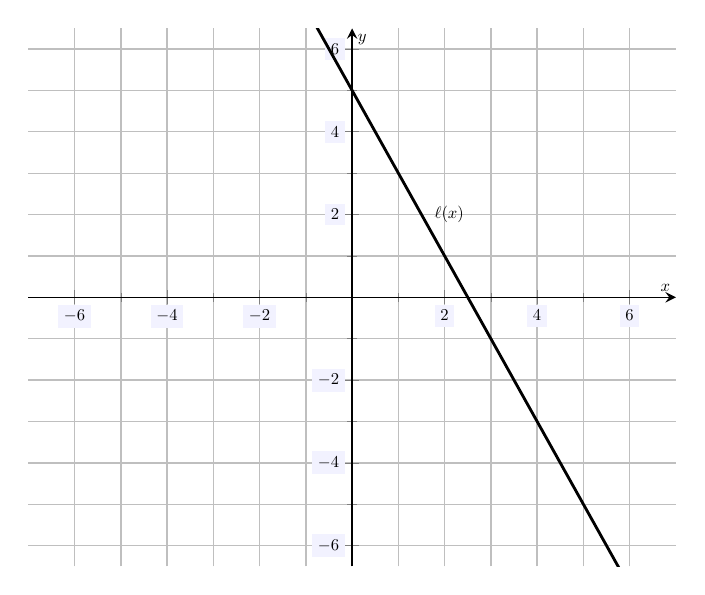
\begin{tikzpicture}[scale=1.2,every node/.style={scale=0.5}]
	\begin{axis}[
	grid=both,
	axis lines=middle,
	ticklabel style={fill=blue!5!white},
	xmin= -7, xmax=7,
	ymin= -6.5, ymax=6.5,
	xtick={-6,-4,-2,0,2,4,6},
	ytick={-6,-4,-2,0,2,4,6},
	minor tick = {-5,-3,...,5},
	xlabel=\(x\),ylabel=\(y\),
	]
	\addplot[domain=-7:7, samples=100,line width=0.03cm] (x,5 - 2*x);
	\node at (2.1,2) {$\ell(x)$};
	\end{axis}
	\end{tikzpicture}
	}
	\]

\begin{enumerate}[(a)]
\item Is $\ell(x)$ a linear function? Explain.
\item Find the equation for $\ell(x)$. 
\item Find the $x$ and $y$-intercepts for $\ell(x)$. 
\item Find a value of $x$ for which $\ell(x)= -3$. 
\end{enumerate} \pspace

\sol 
\begin{enumerate}[(a)]
\item The relation $\ell(x)$ is linear because its graph is a line. \pspace

\item From (a), we know that $\ell(x)$ is linear. Therefore, $\ell(x)= mx + b$ for some $m, b$. Examining the plot above, we can see that $\ell(x)$ contains the points $(0, 5)$, $(1, 3)$, $(2, 1)$, $(3, -1)$, $(4, -3)$, and $(5, 5)$. Using the first two points, we have\dots
	\[
	m= \dfrac{\Delta y}{\Delta x}= \dfrac{5 - 3}{0 - 1}= \dfrac{2}{-1}= -2 
	\]
But then $\ell(x)= mx + b= -2x + b$. But because the line contains the point $(0, 5)$, we have\dots
	\[
	\begin{gathered}
	\ell(0)= -2(0) + b \\
	5= 0 + b \\
	5= b
	\end{gathered}
	\]
Therefore, $\ell(x)= -2x + 5$. 

\item The $x$-intercept for $\ell(x)$ is a value, say $x_0$, for which $f(x_0)= 0$. But then, we have\dots
	\[
	\begin{gathered}
	\ell(x_0)= 0 \\
	-2x_0 + 5= 0 \\
	-2x= -5 \\
	x= 2.5
	\end{gathered}
	\]
Because the steps above are reversible, we know $f(2.5)= 0$. Therefore, the $x$-intercept for $\ell(x)$ is $x= 2.5$, i.e. the points $(2.5, 0)$. We can also see and estimate this in the plot of $\ell(x)$ given above. \pspace

The $y$-intercept for $\ell(x)$ is the point where $\ell(x)$ intersects the $y$-axis. But this is where $x=0$. Then we have $\ell(0)= -2(0) + 5= 0 + 5= 5$. Therefore, the $y$-intercept for $\ell(x)$ is $y= 5$, i.e. the point $(0, 5)$. \pspace

Alternatively, from (b), we know that $\ell(x)= -2x + 5$ has the form $y= mx + b$ with $m= -2$ and $b= 5$. But from (a), we know that $\ell(x)$ is linear so that $b= 5$ must represent the $y$-intercept, i.e. the point $(0, 5)$. \pspace

\item Suppose that there is an $x$, say $x_0$, such that $\ell(x_0)= -3$. But then, we have\dots
	\[
	\begin{gathered}
	\ell(x_0)= -3 \\
	-2x_0 + 5= -3 \\
	-2x_0= -8 \\
	x_0= 4
	\end{gathered}
	\]
As all the steps above are reversible, we know that $\ell(4)= -3$. 
\end{enumerate}



\newpage



% Problem 3
\problem{10} Consider the linear function that goes through the points $(-4, 5)$ and $(6, 0)$.
	\begin{enumerate}[(a)]
	\item Find the slope of this linear function.
	\item Find the equation of this linear function.
	\end{enumerate} \pspace

\sol 
\begin{enumerate}[(a)]
\item We know that $m= \frac{\Delta y}{\Delta x}$. But then\dots
	\[
	m= \dfrac{\Delta y}{\Delta x}= \dfrac{0 - 5}{6 - (-4)}= \dfrac{0 - 5}{6 + 4}= \dfrac{-5}{10}= -\dfrac{1}{2}
	\] \pspace

\item Because $\ell(x)$ is a linear function, we know that $\ell(x)= mx + b$ for some $m, b$. From (a), we know that $m= -\frac{1}{2}$. Then $\ell(x)= -\frac{1}{2}\, x + b$. Because the line contains the point $(-4, 5)$, we know that it satisfies the equation for $\ell(x)$. But then\dots
	\[
	\begin{gathered}
	\ell(-4)= -\dfrac{1}{2} \cdot -4 + b \\
	5= \dfrac{4}{2} + b \\
	5= 2 + b \\
	b= 3
	\end{gathered}
	\]
Therefore, $\ell(x)= -\frac{1}{2}\, x + 3$. 
\end{enumerate}



\newpage



% Problem 4
\problem{10} A certain product requires \$800 of upfront costs to produce---the \textit{fixed costs}. After this investment, it costs \$8.50 produce every item. 
	\begin{enumerate}[(a)]
	\item Explain why the cost to produce $q$ items, $C(q)$, is a linear function.
	\item Find the equation for $C(q)$.
	\item What does the $y$-intercept for $C(q)$ represent?
	\item How much does it cost to produce 10,000~items?
	\item What is the maximum number of items you could produce with \$6,000?
	\end{enumerate} \pspace

\sol 
\begin{enumerate}[(a)]
\item We know that $C(q)$ is a function because given any number of items produced, there is only one total cost of production associated with this production level. We know that $C(q)$ is a linear function because the rate of change of $C(q)$, i.e. the cost of producing additional items, is constant. \pspace

\item From (a), we know that $C(q)$ is linear. Therefore, $C(q)= mq + b$ for some $m, b$. Because the rate of change of $C(q)$, i.e. the cost of producing additional items, is $\$8.50$, we know that $m= 8.50$. But then $C(q)= 8.50q + b$. We know that there are \$800 of upfront costs, i.e. costs before any production of items. We then know that $C(0)= \$800$. This shows\dots
	\[
	\begin{gathered}
	C(0)= 8.50q + b \\
	800= 8.50(0) + b \\
	800= 0 + b \\
	b= 800
	\end{gathered}
	\]
Therefore, $C(q)= 8.50q + 800$. \pspace

\item The $y$-intercept for $C(q)$ is the point where $C(q)$ intersects the $y$-axis. But the $y$-axis is where $q= 0$. Therefore, the $y$-intercept of $C(q)$ is $C(0)= 8.50(0) + 800= \$800$, i.e. the point $(0, \$800)$. Equivalently, because $C(q)$ is linear with $m= 8.50$ and $b= 800$, we know that the $y$-intercept is $b= 800$, i.e. the point $(0, 800)$. This represents the upfront cost of \$800 to produce the items, i.e. the \textit{fixed costs}. \pspace

\item This is precisely $C(10000)$, which is\dots
	\[
	C(10000)= 8.50(10000) + 800= 85000 + 800= \$85,\!800
	\]
Therefore, it costs \$85,800 in total to produce 10,000 items. \pspace

\item One could only produce an amount of items $q$ such that $C(q) \geq \$6,\!000$ with \$6,000. Then we know\dots
	\[
	\begin{gathered}
	C(q) \leq 6000 \\
	8.50q + 800 \leq 6000 \\
	8.50q \leq 5200 \\
	q \leq 611.765
	\end{gathered}
	\]
We assume you can not produce a partial item. So either $q= 611$ or $q= 612$. Clearly, one cannot afford to produce $q=612$~items. Therefore, $q= 611$; that is, one could only afford to produce 611~items. 
\end{enumerate}


\end{document}